\sectionframe{Period-adding in our Model}
\section{Period-adding}

\begin{frame}{Period-adding in our Model}
	\begin{figure}
		\includegraphics[width=.4 \textwidth]{62_MinimalRepr_Adding/2D_Period_1/result.png}
		\quad
		\includegraphics[width=.4 \textwidth]{62_MinimalRepr_Adding/2D_Period_1_Zoomed/result.png}
	\end{figure}
\end{frame}

\begin{frame}{Parameter Changes Needed}
	\vspace{-1em}
	\begin{figure}
		\includegraphics[width=.4 \textwidth]{60_MinimalRepr/Cobweb_E16/result.png}
		\includegraphics[width=.4 \textwidth]{62_MinimalRepr_Adding/Cob_1_ZCorn/result.png}
	\end{figure}
	We got rid of the local minimum on branches $\A$ and $\C$
	\todo{arrow in figure}
\end{frame}

\begin{frame}{The Path to Period-adding}
	\todo{what happens to type B parameter regions}
	\todo{how do period-adding regions open}

	\todo{abstract schematic pictures, then numeric examples}
\end{frame}

\begin{frame}{Describing the Period-adding}
	\vspace{-1em}
	\begin{figure}
		\only<1>{
			\includegraphics[width=.4 \textwidth]{62_MinimalRepr_Adding/2D_Period_1_Zoomed/result.png}
		}
		\only<2>{
			\includegraphics[width=.4 \textwidth]{62_MinimalRepr_Adding/1D_Period_1_add_hor_D1/result.png}
		}
		\only<3>{
			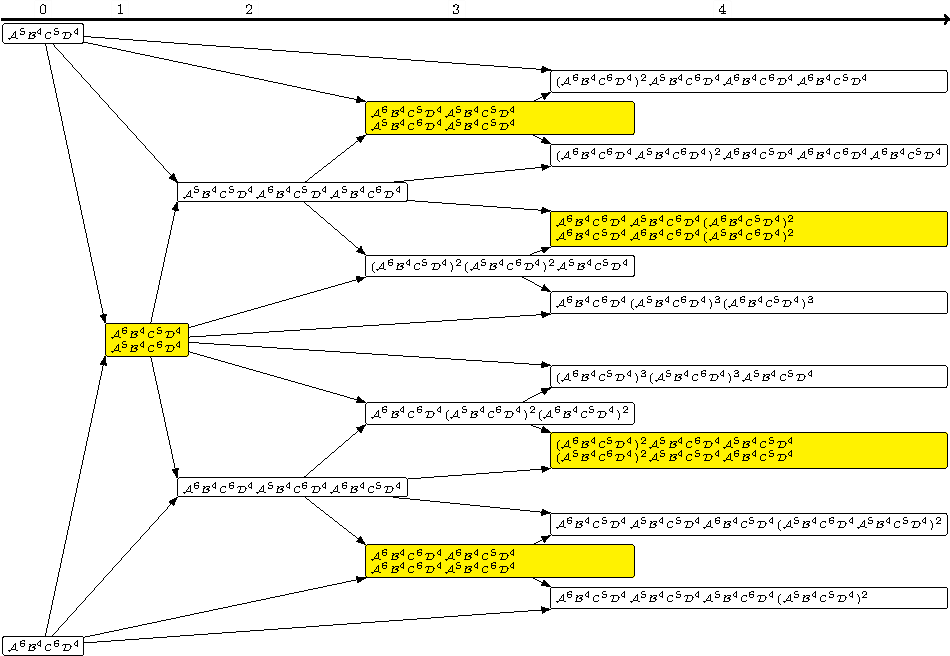
\includegraphics[width=.6 \textwidth]{../../Report/Figures/FareyTrees/Minrep_Adding1_Full/adding.pdf}
		}
	\end{figure}
\end{frame}

\begin{frame}{Problems with the Period-adding}
	\begin{itemize}
		\item Periods don't add
		\item Cycles don't concatenate
	\end{itemize}
	\pause
	\vspace{3em}
	Is this something different entirely?
\end{frame}
